% -*- latex -*-

\chapter{New Worklet Types}
\label{chap:NewWorkletTypes}

\index{worklet types!creating new|(}

The basic building block for an algorithm in \VTKm is the worklet.
Chapter~\ref{chap:Worklets} describes the different types of worklet types provided by \VTKm and how to use them to create algorithms.
However, it is entirely possible that this set of worklet types does not directly cover what is needed to implement a particular algorithm.
One way around this problem is to use some of the numerous back doors provided by \VTKm to provide less restricted access in the execution environment such as using whole arrays for random access.

However, it make come to pass that you encounter a particular pattern of execution that you find useful for implementing several algorithms.
If such is the case, it can be worthwhile to create a new worklet type that directly supports such a pattern.
Creating a new worklet type can provide two key advantages.
First, it makes implementing algorithms of this nature easier, which saves developer time.
Second, it can make the implementation of such algorithms safer.
By encapsulating the management of structures and regulating the data access, users of the worklet type can be more assured of correct behavior.

This chapter documents the process for creating new worklet types.
The operation of a worklet requires the coordination of several different object types such as dispatchers, argument handlers, and thread indices.
This chapter will provide examples of all these required components.
To tie all these features together, we start this chapter with a motivating example for an implementation of a custom worklet type.
The chapter then discusses the individual components of the worklet, which in the end come together for the worklet type that is then demonstrated.

\section{Motivating Example}
\label{sec:NewWorkletTypes:MotivatingExample}

For our motivation to create a new worklet type, let us consider the use case of building fractals.
Fractals are generally not a primary consern of visualization libraries like \VTKm, but building a fractal (or approximations of fractals) has similarities the the computational geometry problems in scientific visualization.
In particular, we consider the class of fractals that is generated by replacing each line in a shape with some collection of lines.
These types of fractals are interesting because, in addition to other reasons, the right parameters result in a shape that has infinite length confined to a finite area.

A simple but well known example of a line fractal is the \index{Koch Snowflake} Koch Snowflake.
The Koch Snowflake starts as a line or triangle that gets replaced with the curve shown in Figure~\ref{fig:KochShape}.

\begin{figure}[htb]
  \centering
  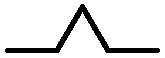
\includegraphics[scale=2]{images/Koch1.pdf}
  \caption{Basic shape for the Koch Snowflake.}
  \label{fig:KochShape}
\end{figure}

The fractal is formed by iteratively replacing the curve's lines with this basic shape.
Figure~\ref{fig:KochIterations} shows the second iteration and then several subsequent iterations that create a ``fuzzy'' curve.
The curve is confined to a limited area regardless of how many iterations are performend, but the length of the curve approaches infinity as the number of iterations approaches infinity.

\begin{figure}[htb]
  \centering
  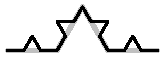
\includegraphics[scale=2]{images/Koch2.pdf}
  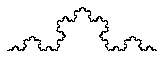
\includegraphics[scale=2]{images/Koch5.pdf}
  \caption{
    The Koch Snowflake after the second iteration (left image) and after several more iterations (right image).
  }
  \label{fig:KochIterations}
\end{figure}

In our finite world we want to estimate the curve of the Koch Snowflake by performing a finite amount of iterations.
The size of the curve grows quickly and in practice it takes few iterations to make close approximations.

\begin{didyouknow}
  The Koch Snowflake is just one example of many line fractals we can make with this recursive line substitution, which is why it is fruitful to create a worklet type to implement such fractals.
  We use the Koch Snowflake to set up the example here.
  Section~\ref{sec:NewWorkletTypes:Using} provides several more examples.
\end{didyouknow}

To implement line fractals of this nature, we want to be able to define the lines of the base shape in terms of parametric coordinates and then transform the coordinates to align with a line segment.
For example, the Koch Snowflake base shape could be defined with parametric coordinates shown in Figure~\ref{fig:KochParametric}.

\begin{figure}[htb]
  \centering
  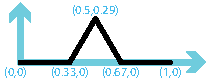
\includegraphics[scale=2]{images/KochParametric}
  \caption{Parametric coordinates for the Koch Snowflake shape.}
  \label{fig:KochParametric}
\end{figure}

Given these parametric coordinates, for each line we define an axis with the main axis along the line segment and the secondary axis perpendicular to that.
Given this definition, we can perform each fractal iteration by applying this transform for each line segment as shown in Figure~\ref{fig:KochApply}.

\begin{figure}[htb]
  \centering
  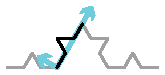
\includegraphics[scale=2]{images/KochApply}
  \caption{Applying the line fractal transform for the Koch Snowflake.}
  \label{fig:KochApply}
\end{figure}

To implement the application of the line fractal demonstrated in Figure~\ref{fig:KochApply}, let us define a class named \textcode{LineFractalTransform} that takes as its constructor the coordinates of two ends of the original line.
As its operator, \textcode{LineFractalTransform} takes a point in parametric space and returns the coordinates in world space in respect to the original line segment.
We define this class in the \vtkmexec{} namespace because the intended use case is by worklets of the type we are making.
A definition of \textcode{LineFractalTransform} is given in Example~\ref{ex:LineFractalTransform}

\vtkmlisting[ex:LineFractalTransform]{A support class for a line fractal worklet.}{LineFractalTransform.h}

\begin{didyouknow}
  The definition of \textcode{LineFractalTransform} (or something like it) is not strictly necessary for implementing a worklet type.
  However, it is common to implement such supporting classes that operate in the execution environment in support of the operations typically applied by the worklet type.
\end{didyouknow}

The remainder of this chapter is dedicated to defining a \textcode{WorkletLineFractal} class and supporting objects that allow you to easily make line fractals.
Example~\ref{ex:KochSnowflake} demonstrates how we intend to use this worklet type.

\vtkmlisting[ex:KochSnowflake]{Demonstration of how we want to use the line fractal worklet.}{KochSnowflake.cxx}

\section{Thread Indices}
\label{sec:ThreadIndices}

\index{thread indices|(}

\fix{\vtkmexecarg{ThreadIndices}}

\index{thread indices|)}

\section{Signature Tags}
\label{sec:NewWorkletTypes:SignatureTags}

\section{Defining the Worklet Superclass}

\section{Dispatcher}
\label{sec:NewWorkletTypes:Dispatcher}

\index{dispatcher!creating new|(}
\index{dispatcher!creating new|)}


\section{Using the Worklet}
\label{sec:NewWorkletTypes:Using}

\fix{Several fun examples.}


\index{worklet types!creating new|)}
